\section{Continual Pre-Training and Scaling Laws}

This section reviews the optimization mechanics of continual pre-training (CPT) and the scaling laws that predict domain adaptation outcomes. Although this work is primarily RAG-centric and freezes the backbone, these results provide the reference framework for any domain-adaptive pre-training (DAP) on Vietnamese legal text and, crucially, a principled method for choosing data mixtures.

\subsection{The Stability Gap and Learning-Rate Schedules}
When pre-training is resumed from a converged checkpoint, the learning rate has decayed to its minimum, and naively continuing causes a \textbf{stability gap}: a temporary but severe validation-loss spike. Gupta et al. \parencite{gupta2023continualpretraininglargelanguage} show that this gap stems from optimizer momentum mismatch (AdamW) rather than data shift, and that \emph{re-warming} the learning rate to its maximum before re-decaying restores plasticity and smooths convergence (Figure~\ref{fig:stability_gap}). Yildiz et al. \parencite{yildiz2025investigatingcontinualpretraininglarge} corroborate that the maximum learning rate governs the plasticity--stability trade-off, while Du et al. \parencite{du2024unlockingcontinuallearningabilities} and Peng et al. \parencite{peng2024scalablelanguagemodelgeneralized} propose gradient- and architecture-level remedies to smooth the gap.

\begin{figure}[H]
\centering
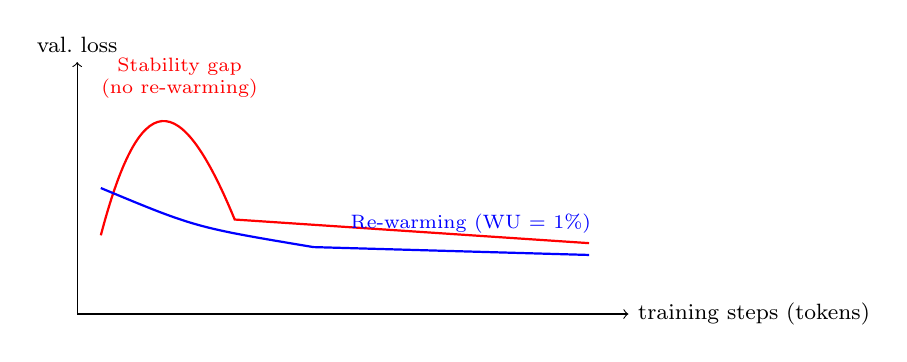
\begin{tikzpicture}[font=\small]
  \draw[->] (0,0) -- (7,0) node[right]{\footnotesize training steps (tokens)};
  \draw[->] (0,0) -- (0,3.2) node[above]{\footnotesize val.\ loss};
  \draw[thick,red] (0.3,1.0) .. controls (0.8,2.9) and (1.3,2.9) .. (2.0,1.2) -- (6.5,0.9);
  \node[red,font=\scriptsize,align=center] at (1.3,3.0) {Stability gap\\(no re-warming)};
  \draw[thick,blue] (0.3,1.6) .. controls (1.5,1.1) .. (3.0,0.85) -- (6.5,0.75);
  \node[blue,font=\scriptsize] at (5.0,1.15) {Re-warming (WU = 1\%)};
\end{tikzpicture}
\caption{Validation loss during continual pre-training with and without learning-rate re-warming \parencite{gupta2023continualpretraininglargelanguage}.}
\label{fig:stability_gap}
\end{figure}

\subsection{Replay Strategies and Distribution Shift}
The required replay budget scales with the severity of the distribution shift. Ibrahim et al. \parencite{ibrahim2024simplescalablestrategiescontinually} introduce \emph{compute-equivalent replay} and show that a weak shift needs only about $5\%$ replay to match a full-retraining baseline at half the compute, whereas Zheng et al. \parencite{zheng-etal-2024-breaking} find that a strong shift---such as a cross-lingual transition---requires $15\%$ to $25\%$ replay to preserve the original linguistic structure. Adapting an English-centric backbone to Vietnamese legal text constitutes a strong shift, implying both a high replay ratio and tokenizer extension.

\subsection{Domain-Specific Scaling Laws}
Que et al. \parencite{que2024dcptlawdomainspecificcontinual} propose the \textbf{D-CPT Law}, which extends the Chinchilla formulation with a domain mixture ratio $r$:
\begin{equation}
L(N, D, r) = E + \frac{A}{N^{\alpha}} + \frac{B \cdot r^{\eta}}{D^{\beta}} + \frac{C}{(r+\epsilon)^{\gamma}} ,
\end{equation}
fitting empirical loss with $R^2 > 0.97$ and enabling prediction of the optimal mixture ratio using only about $1\%$ of the training compute. As Table~\ref{tab:dcpt} shows, for a constrained legal corpus the predicted optimal domain ratio is approximately $0.64$ (i.e. $64\%$ legal and $36\%$ general text), providing a quantitative anchor for the Vietnamese legal setting. Time-continual benchmarks such as TiC-LM \parencite{li2025ticlmwebscalebenchmarktimecontinual} further formalize how knowledge becomes stale over time, which aligns with the temporal-regime requirement of legal knowledge.

\begin{table}[H]
\centering
\small
\caption{D-CPT Law predicted versus real optimal domain mixture ratios \parencite{que2024dcptlawdomainspecificcontinual}.}
\label{tab:dcpt}
\begin{tabularx}{\textwidth}{X c c c}
\hline
\textbf{Constraint setup} & \textbf{Domain} & \textbf{Predicted $r_d$} & \textbf{Real $r_d$} \\
\hline
General loss drift $\le 3\%$ & Chemistry & 0.924 & 0.924 \\
Limited corpus ($D_d = 5\text{B}$) & Music & 0.732 & 0.732 \\
Limited legal corpus ($D_d = 2\text{B}$) & Law & 0.640 & 0.638 \\
\hline
\end{tabularx}
\end{table}

In summary, continual pre-training is feasible but demanding: it requires careful learning-rate re-warming, a substantial replay budget under strong shift, and---ideally---scaling-law-guided mixture selection. These costs, together with the permanent weight modification and forgetting risk discussed earlier, justify positioning CPT as a reference baseline while the proposed framework keeps the backbone frozen and relies on retrieval for factual updates.
